\begin{figure}
    \begin{center}
        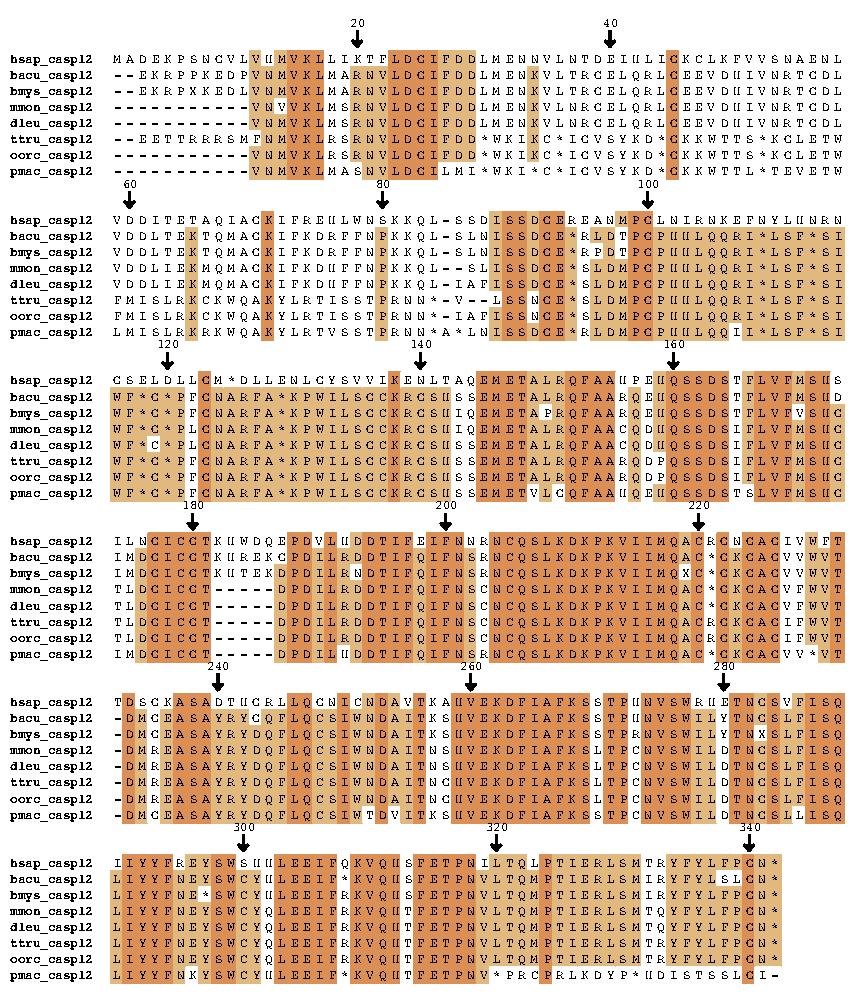
\includegraphics[width=\textwidth]{figures/a_casp12_whole.pdf}
        \caption[Complete alignment of CASP12 in cetaceans]{Complete alignment of CASP12 in cetaceans, showing the complex scheme of evolutive history that lead to its truncation in all cetaceans. Using as reference the truncated human protein referred to in the main text. \hsap; \bacu; \bmys; \mmon; \dleu; \ttru; \oorc; and \pmac.}
        \label{app_f_casp12_align}
    \end{center}
\end{figure}

\begin{figure}
    \begin{center}
        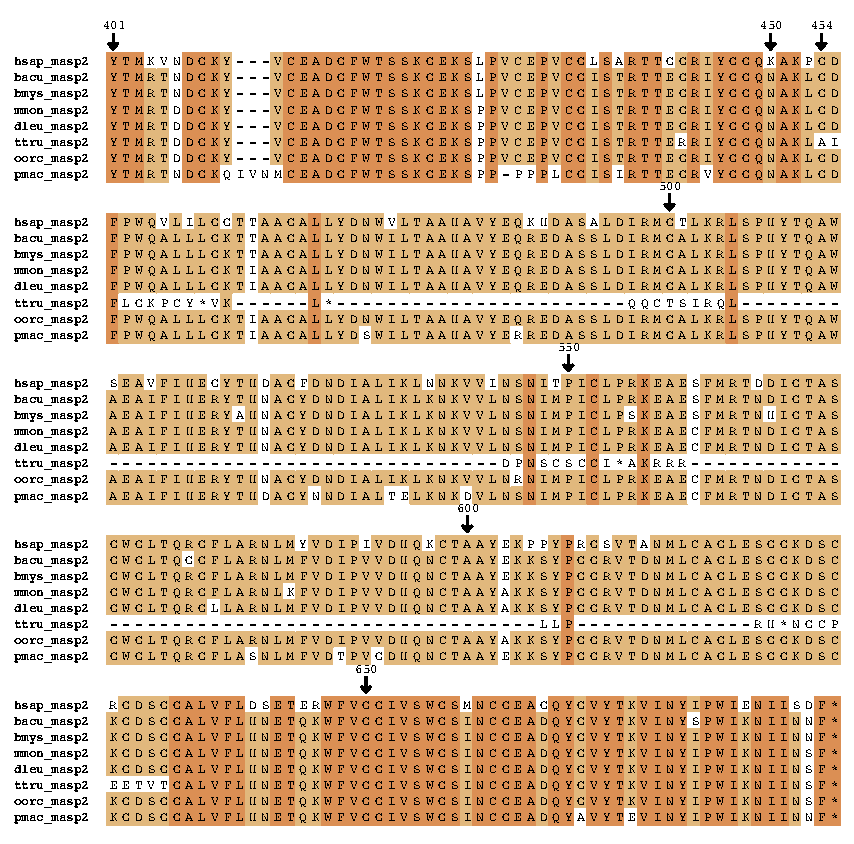
\includegraphics[width=\textwidth]{figures/a_masp2_whole.pdf}
        \caption[Alignment of MASP2 in cetaceans]{Alignment of MASP2 n cetaceans, showing the framshift mentioned in the main text, occurred exclusively on the bottlenose dolphin, starting in {p.G454} and causing several premature stop codons to appear. \hsap; \bacu; \bmys; \mmon; \dleu; \ttru; \oorc; and \pmac.}
        \label{app_f_masp12_align}
    \end{center}
\end{figure}

\begin{figure}
    \begin{center}
        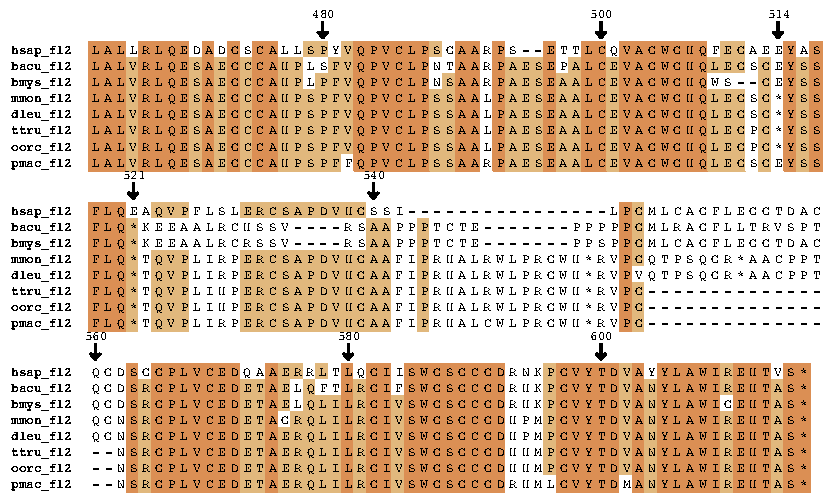
\includegraphics[width=\textwidth]{figures/a_f12_whole.pdf}
        \caption[Alignment of F12 in cetaceans]{Alignment of F12 in cetaceans, showing the different premature stop codons shared by the different groups, caused by different patterns of frameshifts. A different common patter of frameshift can be seen also in the two Misticeti, despite the fact that it does not provoke a premature stop codon as a result. \hsap; \bacu; \bmys; \mmon; \dleu; \ttru; \oorc; and \pmac.}
        \label{app_f_f12_align}
    \end{center}
\end{figure}

\begin{figure}
    \begin{center}
        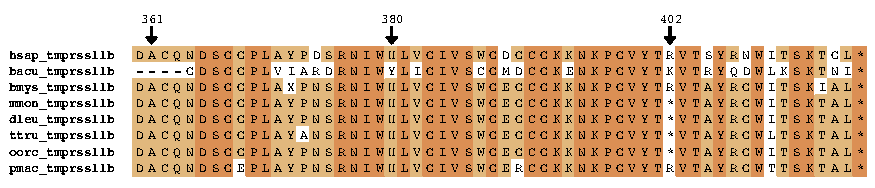
\includegraphics[width=\textwidth]{figures/a_tmprss11b_end.pdf}
        \caption[Alignment of TMPRSS11B in cetaceans, end segment]{Alignment of TMPRSS11B in cetaceans, showing the shared premature stop codon common to all Delphinoidea mentiopned in the main text. \hsap; \bacu; \bmys; \mmon; \dleu; \ttru; \oorc; and \pmac.}
        \label{app_f_tmprss11b_align}
    \end{center}
\end{figure}

\begin{figure}                                                                             
    \begin{center}                                                                             
        \includegraphics[width=\columnwidth]{figures/granzymes.pdf}                            
        \caption[Expansion of the granzyme clusters in \textit{C. abingdonii} and other species]{\footnotesize Expansion of the granzyme clusters in \textit{C. abingdonii} and other organisms (\textit{P. sinensis}, \textit{A. carolinensis}, and \textit{H. sapiens}).}
        \label{app_f_results_george_degradome_granzymes}                                           
    \end{center}                                                                               
\end{figure}
